\chapter{Interazione Radiazione Materia}
Il tempo tipico di decadimento delle particelle dipende dal tipo di interazione:
\begin{itemize}
    \item Forte  < $10^{-22}s$
    \item Debole > $10^{-13}s$
    \item EM $10^{-20}-10^{-14}s$
\end{itemize}
La lunghezza percorsa da una particella prima di decadere è $l=\beta \gamma c \tau_0$ quindi possono essere misurate direttamente protoni, neutroni, elettroni,neutrini (elusivi) e muoni. I $\pi$ e i K possono essere rivelati direttamente ma anche decadere nel rivelatore.
\\
\\
\textbf{Proprietà misurabili} :
\begin{itemize}
    \item \textbf{Momento} : per particelle cariche misurabile tramite il raggio di curvatura in campo magnetico $$p=qRB$$ \begin{center}
        (R ha un segno per essere consistente con la direzione e con la carica)
    \end{center}
    \item \textbf{Carica} : Direzione della deflessione in campo magnetico
    \item \textbf{Energia}: Misurabile tramite la carica rilasciata o la luce prodotta in un calorimetro
    \item \textbf{Tempo di vita}: Ricostruendo il vertice del decadimento (geometricamente) si può ricavare il tempo in cui è decaduta
    \item \textbf{Velocità}: Tramite TOF, angolo Cherenkov o dal $\frac{dE}{dx}$
    \item \textbf{Massa}: Ottenibile da $m^2=E^2-p^2$ o da $p=m\beta/\sqrt{1-\beta^2} $
\end{itemize}

\section{Interazione di particelle cariche}
I meccanismi di interazione principali per le particelle cariche sono:
\begin{itemize}

    \item \textbf{Eccitazione/Ionizzazione}: Un atomo viene ionizzato rilasciando un $e^-$ poi collezionato per formare un segnale o viene prodotta luce tramite de eccitazione

    \item \textbf{Bremstrahlung}: Particella che viene deflessa dal campo EM nucleare e irraggia (*significativa solo per $e^+$ ed $e^{-}$: particelle leggere*)

    \item \textbf{Cherenkov}: Onda d'urto EM prodotta da particelle veloci

    \item \textbf{Radiazione di transizione}: Radiazione emessa quando una particella attraversa un mezzo con indice di rifrazione discontinuo (es. separazione tra vuoto e dielettrico). Questo accade perchè il campo elettrico longitudinale subisce un brusco riarrangiamento che ,in situazioni di energie molto alte, causa irraggiamento

    L'intensità della radiazione è $\propto \gamma$ quindi può essere usata per misurare velocità

\end{itemize}

\subsection{Particelle massive}
    \subsubsection*{Stopping power}
        Lo stopping power è definito come il $-dE/dx$ per unità di densità del materiale quindi è misurata in $MeV cm^2/g$  ed è espresso in funzione di $\beta \gamma=p/m$.
        \\
        Queste curve, se non normalizzate per la massa della particella, possono essere utili per fare particle identification poichè ogni particella segue una curva a se

        \begin{figure}[H]
            \centering
            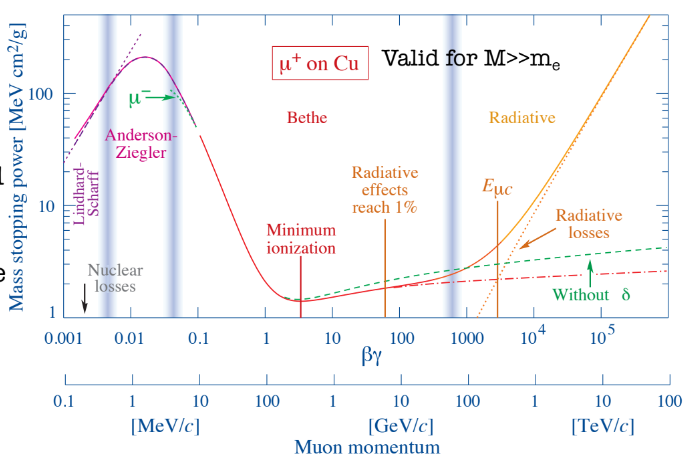
\includegraphics[width=0.8\textwidth,frame]{Chapters/images/Interazione_radiazione_materia/image-20220214171429817.png}
            \caption{Plot dello stopping power per particelle con $M>>m_e$ . Per elettroni e positroni domina Bremstrahlung.\\Possiamo distinguere 3 zone : zona di scattering elastico, di ionizzazione e di Bremstrahlung}
            \label{fig:betheblock}
        \end{figure}
    Analizziamo le diverse regioni della curva:
    \begin{itemize}
        \item Nella zona a più bassa energia (Lindhard-Scharff) si ha un andamento $\propto \beta$ dovuto a scattering elastico su nuclei

        \item La zona di Anderson-Ziegler è ottenuta empiricamente tramite fit su dati sperimentali per mettere un raccordo tra i modelli

        In questa zona si ha l' \textbf{effetto Barkas} che consiste in un minore stopping power per particelle negative (dovuto a fattori correttivi di ordine successivo)

        \item Nella zona di ionizzazione a basse energie si ha un andamento dominato da un fattore cinematico $\sim \beta^{-5/3} \sim \beta^{-2}$ 

        In questa zona la curva è molto sensibile a variazioni di $\beta$ quindi è possibile ricavare la velocità misurando il $dE/dx$

        \item A circa 3 - 4$\beta \gamma$ si ha il minimo di ionizzazione ed è $\sim 1-2 MeV cm^2/g$

        \item Dopo il minimo di ionizzazione si ha una risalita $\propto ln(\beta \gamma)^2$ dovuta all'estensione relativistica del campo elettrico trasversale ma per grandi $\beta \gamma$ il dielettrico viene polarizzato e si ha una saturazione (*effetto del $\delta$*)

        \item Al di sopra dell' \textbf{energia critica} dominano le perdite radiative ovvero la Bremstrahlung e altri processi minori
    \end{itemize}
Concentriamoci un attimo sulle perdite per \textbf{ionizzazione}

\begin{figure}[H]
    \centering
    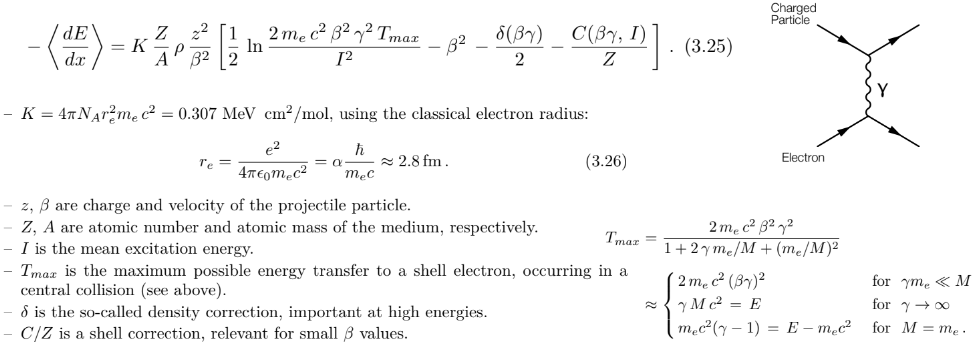
\includegraphics[width=0.95\textwidth,frame]{Chapters/images/Interazione_radiazione_materia/image-20220214173007634.png}
    \captionsetup{width=0.95\linewidth}
    \caption{Bethe-Block: dE/dx dovuta unicamente alla ionizzazione (zona centrale dello stopping power) (e alla radiazione Cherenkov). Non include nè le perdite per bremstrahlung (dominante ad alte energie) nè le perdite per radiazione di transizione}
    \label{fig:betheformula}
\end{figure}





\begin{minipage}{0.48\textwidth}
    \begin{figure}[H]
        \centering
        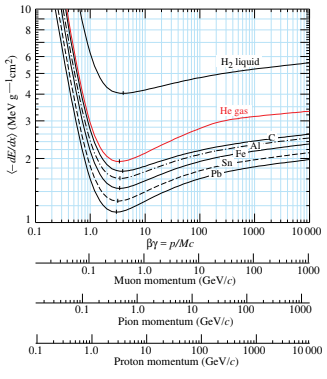
\includegraphics[width=\textwidth,frame]{Chapters/images/Interazione_radiazione_materia/image-20220214175355949.png}
        \captionsetup{width=\textwidth}
        \caption{A: Possiamo vedere come le curve sono essenzialmente indipendenti dal materiale salvo per l'idrogeno. Ricorda che sono normalizzate per la densità}
        \label{fig:}
    \end{figure}
\end{minipage} \hfill
\begin{minipage}{0.48\textwidth}

\begin{figure}[H]
    \centering
    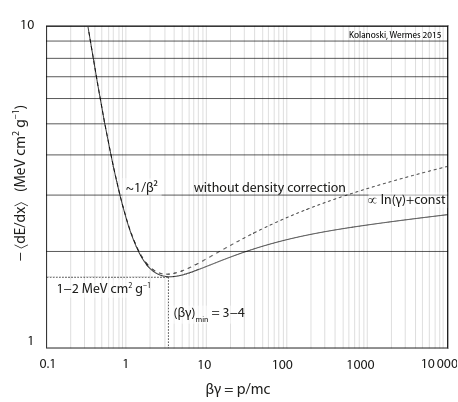
\includegraphics[width=\textwidth,frame]{Chapters/images/Interazione_radiazione_materia/image-20220214175429234.png}
    \captionsetup{width=\textwidth}
    \caption{B: Qui è possibile vedere meglio l'effetto del termine $\delta$ e della dipendenza logaritmica}
    \label{fig:}
\end{figure}

\end{minipage}
Alcune osservazioni sulla Bethe-Block (ionizzazione):
\begin{itemize}
    \item il fattore Z/A, per la formula semiempirica di massa, è più o meno sempre lo stesso $Z/A\sim 0.4$ tranne che per l'idrogeno $H_2$ dove è 1 (poichè non ha neutroni)
    \item A basse energie domina andamento $\sim \beta^{-2}$. 
    \item La curva poi risale per 2 motivi: 
    1. La massima energia trasferibile aumenta con $ \gamma$ (effetto cinematico)
    2. Il campo elettrico trasversale subisce un estensione per effetti relativistici anche se limitato dallo screening degli elettroni atomici che vengono polarizzati (termine $\delta$)
\end{itemize}

\subsubsection*{Picco di Bragg}

\begin{minipage}{0.48\textwidth}
    \begin{figure}[H]
        \centering
        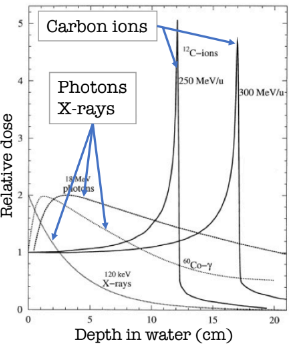
\includegraphics[width=0.75\textwidth,frame]{Chapters/images/Interazione_radiazione_materia/image-20220214183616196.png}
        \captionsetup{width=\textwidth}
        \caption{(La dose non è altro che E/M)}
        \label{fig:braggpeak}
    \end{figure}
\end{minipage} \hfill
\begin{minipage}{0.48\textwidth}
    Man mano che la particella perde energia lo stopping power aumenta. E' possibile ricostruire l'energia persa in funzione della penetrazione usando l'andamento $\beta^{-2}$ valido a basse energie

\end{minipage}

\subsubsection*{Elettroni delta}
Per trasferimenti di energia elevati possono essere strappati elettroni atomici che creano tracce secondarie (sufficientemente lunghe) nella stessa direzione della particella incidente (o comunque a piccoli angoli).
Se il detector non riesce a trattare adeguatamente questi elettroni si può avere un peggioramento della risoluzione spaziale (poichè la carica viene depositata più lontano dal punto di interazione) e fluttuazioni più grandi dello stopping power

\subsubsection*{Range}
Il range è la lunghezza percorsa dalla particella nel materiale $R=\int_{T_0}^0 (\frac{dE}{dx})^{-1} dT$ dove $T_0$ è l'energia cinetica iniziale della particella.

\begin{figure}[H]
    \centering
    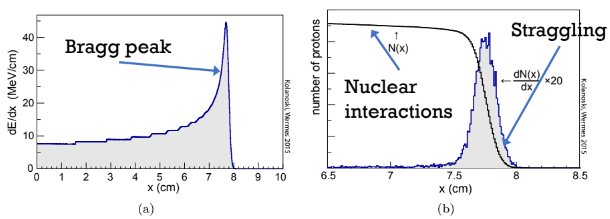
\includegraphics[width=0.8\textwidth,frame]{Chapters/images/Interazione_radiazione_materia/image-20220214185815482.png}
    \captionsetup{width=0.8\linewidth}
    \label{fig:straggling}
\end{figure}


\begin{minipage}{0.48\textwidth}
    \begin{figure}[H]
        \centering
        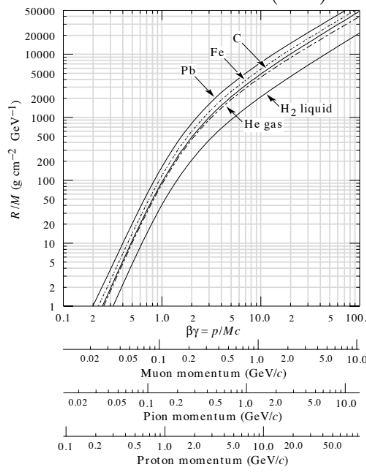
\includegraphics[width=\textwidth,frame]{Chapters/images/Interazione_radiazione_materia/image-20220216172742194.png}
        \captionsetup{width=\textwidth}
        \caption{Range normalizzato per la densità del materiale in funzione di $\beta \gamma$ . Plot utile per capire quanto materiale usare in un esperimento}
        \label{fig:}
    \end{figure}
\end{minipage} \hspace{1.cm}
\begin{minipage}{0.33\textwidth}
    Quando sono coinvolti fenomeni di assorbimento il numero di particelle decresce esponenzialmente (fotoni).
Quando sono coinvolte particelle cariche il numero di particelle rimane pressocchè costante. In figura si vede una lieve diminuzione dovuta a interazioni nucleari.
\\
\\
Si nota anche che il $dN/dx$ non è una delta ma ha una sua larghezza chiamata \textbf{straggling}: questo fenomeno è dovuto alle fluttuazioni statistiche dell'energia rilasciata nel materiale (vedi più avanti)
\\
\\
    Se si esprime l'integrale del range in funzione di $\gamma$ si ha $R=\frac{M}{z^2}f(\gamma_0)$ dove $\gamma_0$ è il $\gamma$ iniziale della particella e $f(\gamma_0)$ è una funzione indipendente dalle proprietà della particella (massa e carica) e dipende solo dal materiale. Quindi il range scala come $M/z^2$ (riferite alla particella)

\end{minipage}
\subsection*{Particelle poco massive ($e^{+} ; e^{-})$}
Per le particelle cariche poco massive (elettroni e positroni) vale quanto detto sopra ma sono presenti dei fenomeni aggiuntivi: 
\begin{itemize}
    

    \item La \textbf{bremstrahlug}  
    \item Gli elettroni incidenti scatterano con elettroni atomici: Sono particelle identiche, interviene il principio di pauli
    \item Per positroni va considerata l'annichilazione con gli elettroni atomici

    Generalmente, oltre a prendere in considerazione la bremstrahlung, vanno considerati 2 regimi di energia:

    \item Quando i livelli energetici degli elettroni atomici NON possono essere trascurati si fa la media come nel caso di particelle massive
    \item Quando si hanno grandi trasferimenti di energia vengono considerati gli scattering Moller ($e^- e^- \to e^- e^-$) e Bhabha ($e^+ e^- \to e^+ e^-$)  
\end{itemize}

\begin{figure}[H]
    \centering
    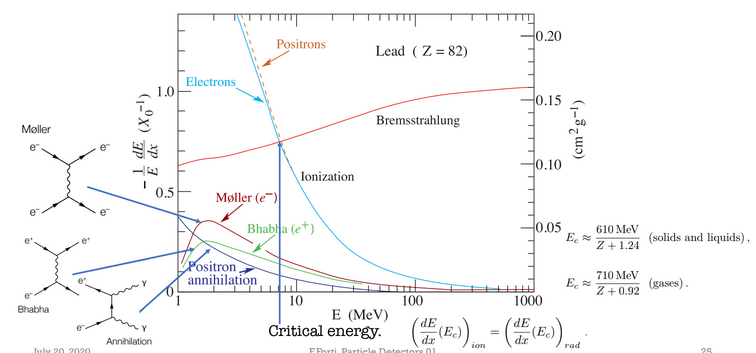
\includegraphics[width=0.8\textwidth,frame]{Chapters/images/Interazione_radiazione_materia/image-20220217021527324.png}
    \captionsetup{width=0.8\linewidth}
    \caption{Per particelle leggere il dE/dx è molto diverso in quanto la bremmstrahlung diventa dominante già sotto il GeV, nel piombo già a 7MeV \\ Anche qui si nota l'effetto per il quale la particella con carica negativa a basse energie perde un po' meno energia}
    \label{fig:electronloss}
\end{figure}
\subsubsection*{Bremstrahlung e lunghezza di radiazione}
Consiste nell'irragiamento dovuto alla deflessione dell'elettrone causata dal campo elettrico nucleare (scattering Rutherford con il nucleo)
\newline
L'energia emessa per una carica accelerata, sia nel limite classico che quantistico, è $dE/dt \propto \frac{1}{m^2}$

\begin{note}
    Ad altissime energie (es. LHC) la bremmstrahlung diventa rilevante anche per muoni e pioni
\end{note}